	\documentclass[10pt,oneside]{CBFT_book}
	% Algunos paquetes
	\usepackage{amssymb}
	\usepackage{amsmath}
	\usepackage{graphicx}
	\usepackage{libertine}
	\usepackage[bold-style=TeX]{unicode-math}
	\usepackage{lipsum}

	\usepackage{natbib}
	\setcitestyle{square}

	\usepackage{polyglossia}
	\setdefaultlanguage{spanish}
	



	\usepackage{CBFT.estilo} % Cargo la hoja de estilo

	% Tipografías
	% \setromanfont[Mapping=tex-text]{Linux Libertine O}
	% \setsansfont[Mapping=tex-text]{DejaVu Sans}
	% \setmonofont[Mapping=tex-text]{DejaVu Sans Mono}

	%===================================================================
	%	DOCUMENTO PROPIAMENTE DICHO
	%===================================================================

\begin{document}

% =================================================================================================
\chapter{Dinámica cuántica}
% =================================================================================================

Queremos ver la evolución temporal de los kets 
\[
	\Ket{\alpha,t_0,t},
\]
notación que refiere al estado $\alpha$ que partió en $t_0$ al tiempo $t$. Pictóricamente
\[
	\Ket{\alpha,t_0} \underbrace{\longrightarrow}_{\text{evoluciona}} \Ket{\alpha,t_0,t}
\]

Emplearemos para ello un operador de evolución temporal $U_{(t,t_0)}$ al cual le pediremos
\[
	\Ket{\alpha,t_0,t} = U \Ket{\alpha,t_0}
\]
con las propiedades

\begin{itemize}
 \item Unitariedad
 \[
	\Braket{ \alpha,t_0,t| \alpha,t_0,t} = 1 \forall t
 \]
 \[
	\Braket{ \alpha,t_0| U^\dagger U| \alpha,t_0} = 1 \quad \Rightarrow \quad 
	U^\dagger U = U U^\dagger = \mathbb{1}
 \]
 para conservación de la probabilidad.
 \item Linealidad
 \[
	U(t_2,t_0) = U(t_2,t_1) U(t_1,t_0) \qquad t_2>t_1>t_0
 \]
 \item Límite a $\mathbb{1}$
 \[
	U_{(t,t_0)} \to \mathbb{1} \quad \text{si} \quad t\to t_0
 \]
 o bien 
 \[
	U_{(t_0+dt,t_0)} \to \mathbb{1} \quad \text{si} \quad dt\to 0
 \]
\end{itemize}

Se propone entonces un 
\[
	U_{(t+dt,t)} = \mathbb{1} - i\Omega dt 
\]
con $\Omega$ hermítico. Comparando con clásica vemos que $H$ origina la evolución temporal, entonces
identificamos $\Omega$ con $H$, del modo $\Omega = H/\hbar$ así que 
\[
	U_{(t+dt,t)} = \mathbb{1} - \frac{i}{\hbar} H dt .
\]

De esta forma 
\[
	U_{(t+dt,t_0)} =  U_{(t+dt,t)} U_{(t,t_0)}  = \left( \mathbb{1} - \frac{i}{\hbar} H dt \right) U_{(t,t_0)}
\]
\[
	\dpar{U}{t} = \frac{ U_{(t+dt,t_0)} - U_{(t,t_0)} }{dt} = - \frac{i}{\hbar}H U_{(t,t_0)}
\]
y entonces 
\[
	i\hbar\dpar{U}{t} = HU
\]
que es la ecuación para $U_{(t,t_0)}$.
\[
	i\hbar\dpar{}{t} U_{(t,t_0)} \Ket{\alpha,t_0} = H U_{(t,t_0)} \Ket{\alpha,t_0}
\]
y arribamo a la ecuación de Schrödinger para kets
\[
	i\hbar\dpar{}{t} \Ket{\alpha,t_0,t} = H \Ket{\alpha,t_0,t}
\]
donde el inconveniente es que $H=H(t)$.

El concepto se ilustra en la figura siguiente
\begin{figure}[htb]
	\begin{center}
	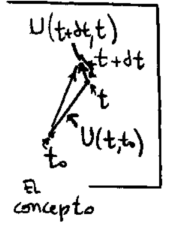
\includegraphics[width=0.3\textwidth]{images/teo2_5.pdf}	 
	\end{center}
	\caption{}
\end{figure} 



% =================================================================================================
\section{Dinámica cuántica}
% =================================================================================================

\subsection{Casos de solución de $U(t,t_o)$}

\begin{itemize}
 \item Supongamos $ H \neq H(t)$, entonces
 \[
	U( t, t_0) = \euler^{-i/\hbar H (t-t_0)} 
 \]
 \item Sea $ H = H(t)$, entonces
 \[
	U( t, t_0) = \euler^{-i/\hbar \int_{t_0}^t H(t')dt'} 
 \]
 y la integral puede hacerse una vez conocida la expresión de $H(t)$.
 \item Sea $ H = H(t)$ con $[H(t_1),H(t_2)] \neq 0$ entonces
 \begin{multline*}
	U( t, t_0) =  1 + \sum_{n=1}^{\infty} \left( \frac{-i}{\hbar}\right)^n 
		\int_{t_0}^t dt_1 \int_{t_0}^{t_1} dt_2 \int_{t_0}^{t_2} dt_3 ... \times \\
			\int_{t_0}^{t_{n-1}} dt_n H(t_1) H(t_2) ... H(t_n)    
 \end{multline*}
%  \[
% 	U( t, t_0) =  1 + \sum_{n=1}^{\infty} \left( \frac{-i}{\hbar}\right)^n 
% 		\int_{t_0}^t dt_1 \int_{t_0}^{t_1} dt_2 \int_{t_0}^{t_2} dt_3 ... \int_{t_0}^{t_{n-1}} dt_n 
% 			H(t_1) H(t_2) ... H(t_n)  
%  \]
 y esta es la serie de Dyson (del físico Freeman Dyson().)
\end{itemize}

El problema que suscita es debido a que si $H$ a diferentes tiempos no conmuta no podemos poner la exponencial en serie 
de potencias. En realidad $\exp({\square})$ tiene sentido sólo si la serie 
\[
	\sum_{n=0}^{\infty}  \frac{1}{n!}\square^n
\]
tiene sentido; es decir, si no surgen ambigüedades al tomar la potencia $n$-ésima del operador $\square$.
\notamargen{El operador $\square$ no se deja poner sombreros, quiere andar con la cabeza descubierta}

Para el caso 1 es simplemente 
 \[
	a
 \]
pero para el caso 3 es 
 \[
	a
 \]
puesto que al operar es 
\[
	a
\]
pues $[H(t'),H(t'')]\neq 0$. En el caso 2 $(\int_{t_0}^t H(t')dt' )^n$ no tiene problemas puesto que está provista la 
conmutatividad.

\subsection{Soluciones útiles}

Primeramente conseguimos un $\hat{A}$ tal que $[ A, H ]=0$ y entonces (estoy considerando $ H \neq H(t)$ )
\[
	a,
\]
luego 
\[
	a
\]
con $\hat{H}$ y $\hat{A}$ conmutan se tiene
\[
	a
\]

Entonces operamos con el $H$ para 
\[
	a
\]
y así 
\[
	a
\]
de manera que comparando con 
\[
	a
\]
El coeficiente es el mismo pero le hemos sumado una fase $\exp(-iE_{a'}(t-t_0)/\hbar)$ que no es global.

\subsection{Evolución de valores de expectación}

Recordemos primeramente que los autoestados no evolucionan. Luego 
\[
	a
\]

La fase es global es considerar una autoestado. La podemos descartar (setear igual a uno)
\[
	a
\]

El valor de expectacion de un operador respecto a un autoestado no varía.
\[
	a
\]
\[
	a
\]
\[
	a
\]

El valor de expectación de un operador respecto a un estado general tiene una fase no global que produce términos de 
interferencia.

\subsection{Relaciones de conmutación}

\[
	[ A + B, C] = [A, C] + [B,C] 
\]
\[
	[A, B] = - [B,A]
\]
\[
	[A, B\cdot C] = B[A,C] +  [A,B]C
\]
\notamargen{Acá no es baca + caballo puesto que no conmutan.}
\[
	i\hbar[ A, B]_{\text{classic}} = [A, B]
\]
donde $[ , ]_{\text{classic}}$ es el corchete de Poisson.
Las relaciones de conmutación fundamentales son 
\[
	[x_i, x_j] = 0 \qquad [p_i, p_j]=0 \qquad [x_i,p_j] =i\hbar\delta_{ij}
\]
a las que podemos sumar
\[
	[x,f(p)] = i\hbar\dpar{f}{p} \qquad [p,G(x)] = i\hbar\dpar{G}{x} 
\]
\[
	[S_i,S_j] = i\hbar \varepsilon_{ijk}S_k
\]

\subsection{La ecuación de Schrödinger}

\[
	a \text{con} \qquad \hat{H} = \frac{\hat{p}^2}{2m} + V(\hat{x}) 
\]
Puedo meter un bra $\Bra{x'}$ que no depende del tiempo y entonces 
\[
	a
\]
\[
	a
\]
de manera que resulta la ecuación de Schrödinger
\[
	a .
\]

\subsection{Representación de Heisenberg}

Los kets y los operadores no tienen sentido físico, pero sí los valores de expectación : toda física podrá modificar 
los primeros pero debe conservar los valores de expectación. Así tenemos dos representaciones posibles:

\begin{center}
\begin{tabular}{|l|l|}
\hline
Schrödinger & Heisenberg \\
\hline
& \\
$\Ket{\alpha} \to U\Ket{\alpha} \quad $ & $\Ket{\alpha} \to \Ket{\alpha} \quad $ \\
& \\
$A \to A \quad $ & $A \to U^\dagger AU \quad$ \\
& \\
$\Ket{a'} \to \Ket{a'} \quad $ & $\Ket{a'} \to U^\dagger \Ket{a'} \quad $ \\
& \\
\hline
\end{tabular}
\end{center}
Así vemos que en Schrödinger los kets evolucionan y los operadores permanecen fijos; al igual que los autoestados.
En cambio en Heisenberg los kets no evolucionan pero sí lo hacen los operadores y los autoestados.

Deben notars que:
\begin{enumerate}
 \item Los productos internos no cambian con el tiempo
 \[
	a
 \]
 \item Los valores de expectacion son los mismos en ambos esquemas
 \[
	a
 \]
 \[
	\Braket{A}^{(S} = \Braket{A}^{(H} \qquad A(t)^H = U(t)^\dagger A^S U(t)
 \]
\end{enumerate}

El operador $\hat{A}$ en Schrödinger no depende explícitamente del tiempo. La idea es que le ``pegamos'' a los 
operadores la evolución temporal de los kets.
\[
	a
\]
pero a $t=t_0$ las representaciones coinciden,
\[
	a
\]

\subsubsection{La ecuación de Heisenberg}

\[
	a
\]
\[
	\Rightarrow 
\]
\[
	a
\]
\[
	a
\]
\[
	a
\]
y llegamos a la ecuación de Heisenberg
\[
	\dpar{A^{(H)}}{t} = \frac{1}{i\hbar} [ A^{(H)}, H^{(H)}]
\]
si $A^{(H)}$ conmuta con el $H^{(H)}$, entonces $A^{(H)}$ es una cantidad conservada (una constante de movimiento).
En ese caso el operador no depende del tiempo y entonces $A^{(H)} = A^{(S)}$.

\subsubsection{Evolución de autoestados}

\[
	a,
\]
aplico un $U^\dagger$ a ambos lados y entonces 
\[
	a
\]
los $a'$ no dependen de la representación porque tienen significado físico. Entonces los $\Ket{a'}$ evolucionan
\[
	a
\]
\[
	a
\]
\[
	a
\]
puesto que recordemos, nota importante,
\[
	a
\]
entonces $H$ es el mismo en ambas puesto que $\hat{U} =\hat{U}(\hat{H}) $ y $[U,H]=0$.

De esta forma los autoestados evolucionan al revés 
\[
	a
\]

Podemos ver de otro modo la equivalencia
\[
	a
\]
pero 
\[
	a
\]
\[
	a
\]

\subsubsection{Coeficientes}

Los coeficientes en Schrödinger y en Heisenberg son 
\[
	a
\]
Entonces en Schrödinger es 
\[
	a
\]
mientras que en Heisenberg es 
\[
	a
\]

Los coeficientes en las expresiones son iguales como corresponde a todo magnitud que tiene sentido físico, pues 
$|c_a(t)|^2$ es la probabilidad.

\subsection{Teorema de Ehrenfest}

Para una partícula libre, donde $p(t)=p(0)$ es constante de movimiento,
\[
	x^{(H)} = x(0) + \frac{p(0)}{m}t
\]
y se tiene 
\[
	[x(t),x(0)] = -\frac{i\hbar}{m}t
\]
\[
	H = \frac{p^2}{2m} + V(x)
\]
\[
	\dtot{P}{t} = \frac{1}{i\hbar}[p,H] = \frac{1}{i\hbar}[p,V(x)] = 
	\frac{1}{i\hbar}\left( -i\hbar\dpar{V}{x}\right),
\]
de modo que 
\[
	\dtot{P}{t} = -\dpar{V}{x} \qquad \longrightarrow \quad m \dtot[2]{x}{t} = -\dpar{V}{x} 
\]
\[
	p = m \dtot{x}{t} \qquad \dtot{p}{t} = m \dtot[2]{x}{t} 
\]
donde estamos usando 
\[
	\dpar{A^H}{t} = \frac{1}{i\hbar}[A^H,H]
\]

Es necesario remarcar que relaciones como $[x,p]=i\hbar$ son para operadores en la picture de Schrödinger, donde los 
operadores no cambian en el tiempo. Estamos en efecto haciendo $[x(0),p(0)]=i\hbar$
\[
	\Braket{\alpha,t_0|m \dtot[2]{x}{t}|\alpha,t_0} = - \Braket{\alpha,t_0|\dpar{V}{x}|\alpha,t_0}
\]
\[
	m\dpar[2]{}{t}\Braket{\alpha,t_0| x^H |\alpha,t_0} = -\Braket{\alpha,t_0|\dpar{V}{x}|\alpha,t_0}
\]
y entonces el teorema de Ehrenfest es 
\[
	m \dpar[2]{}{t} \Braket{x^{(s)}} = - \Braket{ \dpar{V^{(s)}}{x}}
\]
los valores de expectación son iguales en ambas representaciones.
% 
% =================================================================================================
\section{El oscilador armónico}
% =================================================================================================

Para el oscilador armónico 1D  el hamiltoniano y energía eran
\[
	H = \frac{p^2}{2m} + \frac{m\omega^2 x^2}{2} \qquad E = \hbar \omega \left( n + \frac{1}{2} \right)
\]
pero este problema puede resolverse usando un nuevo operador $\hat{a}$
\[
	\hat{a} = \sqrt{\frac{m\omega}{2\hbar}}\left( x + i\frac{p}{m\omega} \right) \qquad \text{con} \quad 
	\hat{a}^\dagger = \sqrt{\frac{m\omega}{2\hbar}}\left( x - i\frac{p}{m\omega} \right)
\]
que es suma de $\hat{x}, \hat{p}$ pero que no es hermítico. Cumple que 
\[
	[a , a^\dagger ] = 1 \qquad a a^\dagger =  \frac{H}{\hbar\omega} -1 \qquad 
	H = \hbar\omega \left( a a^\dagger + \frac{1}{2} \right),
\]
donde se define el operador número $\hat{N}\equiv a^\dagger a$ que al verificar $[\hat{N},\hat{H}]=0$ tienen base de 
autoestados en común $\{ \Ket{n} \}$. En efecto 
\[
	\hat{N} \Ket{n} = n\Ket{n} \qquad
	\hat{H} \Ket{n} = \hbar\omega \left( n + \frac{1}{2} \right) \Ket{n}
\]
siendo $n$ el número de cuantos de energía.
Se cumplen además 
\[
	[N,a] = [a^\dagger a,a] = - [ a, a^\dagger a ] = - \left( a^\dagger [a,a] + [a,a^\dagger]a \right) =
	-a
\]
\[
	[N,a^\dagger] = [a^\dagger a, a^\dagger ] = - [a^\dagger , a^\dagger a ] =
	- \left( a^\dagger [a^\dagger,a] + [a^\dagger,a]a^\dagger \right) = a^\dagger
\]

Queremos ver que le  hace $a^\dagger$  a un autoestado $\Ket{n}$ y luego $a$ sobre el mismo.
\[
	N a^\dagger \Ket{n} = ([N, a^\dagger] + a^\dagger N) \Ket{n} =
	a^\dagger \Ket{n} + a^\dagger n \Ket{n} 
\]
\[
	\Hat{N} (a^\dagger\Ket{n}) = (n+1)(a^\dagger\Ket{n})
\]
Entonces, como no hay degeneración y tenemos $N\Ket{n'} = n'\Ket{n'}$ entonces 
\[
	a^\dagger \Ket{n} = c_1 \Ket{n+1},
\]
y procediendo de modo idem para $a\ket{n}$ será
\[
	a \Ket{n} = c_2 \Ket{n-1}
\]
Luego,
\[
	a^\dagger \Ket{n} = c_1 \Ket{n+1} \overbrace{\longrightarrow}^{DC} 
	\Bra{n+1} c_1^* = \Bra{n} a 
\]
\[
	a \Ket{n} = c_2 \Ket{n-1} \overbrace{\longrightarrow}^{DC} \Bra{n-1} c_2^* = \Bra{n} a^\dagger
\]
y entonces 
\[
	\Braket{n|N|n} = n \Braket{n|n} = n =  \Braket{n| a^\dagger a |n} =  \Braket{n-1|c_2^* c_2|n-1} =
	|c_2|^2 \Braket{n-1|n-1}
\]
\[
	n = \Braket{n|aa^\dagger-1|n} = -1 + \Braket{n|aa^\dagger|n} = - 1 + \Braket{n+1|c_1^*c_1|n+1} =
	-1 + |c_1|^2 \Braket{n+1|n+1}
\]
siendo
\[
	|c_2| = \sqrt{n} \qquad |c_1| = \sqrt{n+1} 
\]
\[
	\hat{a}^\dagger \Ket{n} = \sqrt{n+1} \Ket{n+1} \qquad  \hat{a}\Ket{n} = \sqrt{n} \Ket{n-1} 
\]
y entonces de esta forma $\hat{a}^\dagger$ es el operador de creación de cuantos y $\hat{a}$ el de aniquilación.

\subsection{El estado fundamental $\Braket{0}$}

\[
	a \Ket{n}  \overbrace{\longrightarrow}^{DC} \Bra{n} a^\dagger
\]
y desde el postulado para productos internos,
\[
	(\Bra{n}a^\dagger)(a\Ket{n}) \geq 0 \quad n \Braket{n|n} \geq 0 \Rightarrow n \geq 0 
\]
entonces $n$ cabalga por los naturales.
Si hacemos 
\[
	a\Ket{n} = \sqrt{n} \Ket{n-1}, \qquad  a^2 \Ket{n} = \sqrt{n}\sqrt{n-1} \Ket{n-2} \; ...
\]
en algún momento se llega a $\Ket{n=0}$, entonces $E_0 = \hbar\omega/2$ y 
\[
	\Ket{0} \equiv \text{El fundamental}
\]
y no se puede bajar más,
\[
	\hat{a}\Ket{0} = 0.
\]

Por otra parte, con el $\hat{a}^\dagger$ se puede llegar a cualquier estado
\[
	a^\dagger \Ket{0} = \sqrt{1} \Ket{1}, \qquad  a^{\dagger 2} \Ket{0} = \sqrt{1}\sqrt{2} \Ket{2} = 
	\sqrt{1}\sqrt{2}\sqrt{3} \Ket{3}
\]
\[
	\frac{{(a^{\dagger})}^n}{\sqrt{n}!} \Ket{0} = \Ket{n}
\]

Las matrices de $\hat{a},\hat{a}^\dagger$ sólo tienen una diagonal corrida de elementoss 
\[
	\Braket{n'|a|n} = \sqrt{n} \Braket{n'|n-1} = \sqrt{n} \delta_{n',n-1}
\]
\[
	\Braket{n'|a^\dagger|n} =  \sqrt{n-1} \Braket{n'|n+1} = \sqrt{n-1} \delta_{n',n+1}
\]

También puede verse que 
\[
	\Braket{n|x|n}= 0 \qquad \Braket{n|p|n}= 0
\]
y por ello 
\[
	\Braket{(\Delta x)^2}_{\Ket{0}} \Braket{(\Delta p)^2}_{\Ket{0}} = \frac{\hbar^2}{4} 
\]
el estado fundamental es el de incerteza mínima.

\subsection{Función de onda}

Siendo $\Psi_n(x') = \Braket{x'|n}$ quiero evaluar $\Psi_0(x') = \Braket{x'|0}$ y ver que como 
\[
	\Braket{x'|a|0}= 0 
\]
tengo 
\[
	0 = \sqrt{ \frac{m\omega}{2\hbar} } \Braket{x'|x+\frac{ip}{m\omega}|0} =
	\sqrt{ \frac{m\omega}{2\hbar} } \left[ x'\Braket{x'|0} + \frac{i}{m\omega}\Braket{x'|p|0} \right]
\]
\[
	x' \Braket{x'|0} + \frac{i}{m\omega} (-i\hbar) \dpar{}{x} \Braket{x'|0} = 0
\]
entonces 
\[
	x' \Braket{x'|0} = - \frac{\hbar}{m\omega} \dpar{}{x'}\Braket{x'|0} 
\]
\[
	- \int \frac{m\omega}{\hbar} x' dx' = \int \frac{d \Braket{x'|0}}{\Braket{x'|0}} \Rightarrow 
	\Braket{x'|0} = \kappa \euler^{-m\omega x^{'2}/(2\hbar)}
\]
y entonces 
\[
	1 = \int_{-\infty}^{\infty} \Braket{0|x'}\Braket{x'|0} dx' = 
	\int_{-\infty}^{\infty} |\kappa|^2 \euler^{-m\omega x^{'2}/\hbar} dx' =
	|\kappa|^2 \sqrt{\frac{\pi\hbar}{m\omega}} 
\]
\[
	|\kappa| = \left( \frac{m\omega}{\pi\hbar} \right)^{1/2} = \frac{1}{(\pi x_0^2)^{1/4}}
\]
donde usamos el conocido resultado $\int_{-\infty}^\infty \exp( - a x^2) dx = \sqrt{\pi/a}$, llegamos al llamado pack 
gaussiano.
\[
	\Braket{x'|0} = \frac{1}{(\pi x_0^2)^{1/4}} \euler^{-\frac{1}{2}\left( x'/x_0 \right)^2}
\]
El estado fundamental tiene incerteza mínima y debe corresponder a un paquete gaussiano.

Notemos que $\hat{a}^\dagger$ crea sobre ket y aniquila sobre bra, mientras que $\hat{a}$ aniquila sobre ket y crea 
sobre bra,
\[
	a^\dagger \Ket{n} = \sqrt{n+1} \Ket{n+1} \Rightarrow \Bra{n} a = \Bra{n+1} \sqrt{n+1}
\]
\[
	a \Ket{n} = \sqrt{n} \Ket{n-1} \Rightarrow \Bra{n} a^\dagger = \Bra{n-1} \sqrt{n}
\]

\subsection{Interferencia en experimento de Young}

Consideremos la situación depicted en la figura bajo estas líneas

\begin{figure}[htb]
	\begin{center}
	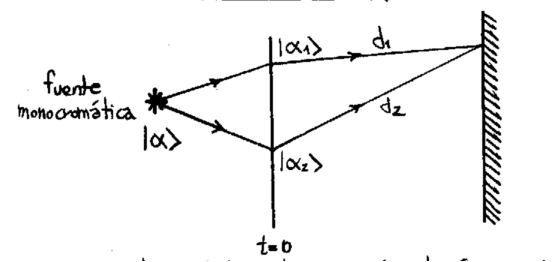
\includegraphics[width=0.6\textwidth]{images/teo2_6.pdf}	 
	\end{center}
	\caption{}
\end{figure} 

Uso $\hat{H}$ de partículas libres.
\[
	\frac{1}{2} \Ket{\alpha} = \Ket{\alpha_1} = \Ket{\alpha_2}
\]
para $t>0$ se tiene 
\[
	\Ket{\tilde{\alpha_1}} = \euler^{ -i H t /\hbar } \Ket{\alpha_1} =
		\euler^{ -i E_\alpha t /\hbar } \Ket{\alpha_1}	
\]
\[
	\Ket{\tilde{\alpha_2}} = \euler^{ -i E_\alpha t /\hbar } \Ket{\alpha_2}	
\]

En la pantalla debe verse la interferencia de los dos estados solapados.
\[
	\Ket{\tilde{\alpha}} = \Ket{\tilde{\alpha_1}} + \Ket{\tilde{\alpha_2}} =
		\euler^{ -i E_\alpha \frac{d_1}{v} /\hbar } \Ket{\alpha_1} +
		\euler^{ -i E_\alpha \frac{d_2}{v} /\hbar } \Ket{\alpha_2}	
\]
\[
	\Ket{\tilde{\alpha}} = \frac{1}{2} \euler^{ -i E_\alpha \frac{d_1}{v} /\hbar } 
		| 1 + \euler^{ -i E_\alpha \frac{d_2-d_1}{v} /\hbar } | \Ket{\alpha_1}
\]
y si definimos
\[
	\beta=E_\alpha \frac{d_2-d_1}{v} /\hbar,
\]
resulta entonces
\[
	\Braket{\tilde{\alpha}|\tilde{\alpha}} = \frac{1}{4}| 1 +  \euler^{ -i E_\alpha \frac{d_2-d_1}{v} /\hbar } |^2 =
		\frac{1}{4}( (1+\cos\beta)^2 + \sin^2\beta ) =
			\frac{1}{2} + \frac{1}{2}\cos\left( \beta \right).
\]


Al partir el estado $\Ket{\alpha_1} $ y volver a unirlo en $\Ket{\alpha_1} + \Ket{\alpha_2}$ vemos una intensidad que 
dependa de la diferencia de camino.

\subsection{Cambio de cero del potencial}

En mecánica clásica la física de un problema no se ve afectada por un cambio de gauge.
Si movemos el cero de potencial, la situación física es la misma.
Veamos qué sucede en mecánica cuántica.
\[
	\Ket{\alpha,t,t_0} = \euler^{ -i (p^2/2m + V(x))(t-t_0)/\hbar} \Ket{\alpha,t_0}
\]
\[
	\Ket{\tilde{\alpha},t,t_0} = \euler^{ -i (p^2/2m + V(x) + V_0)(t-t_0)/\hbar} \Ket{\alpha,t_0}
\]
\[
	\Ket{\tilde{\alpha},t,t_0} = \euler^{ -i V_0(t-t_0)/2 }\Ket{\alpha,t,t_0}
\]
y entonces vemos que $\Ket{\tilde{\alpha},t}$ y $\Ket{\alpha,t}$ difieren en una fase, de manera que los valores de 
expectación no cambian (con $V_0$ constante).

\begin{figure}[htb]
	\begin{center}
	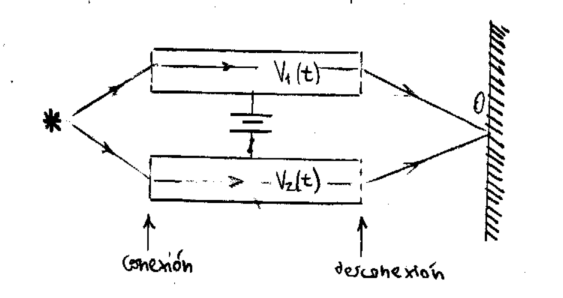
\includegraphics[width=0.6\textwidth]{images/teo2_7.pdf}	 
	\end{center}
	\caption{}
\end{figure} 

Este es un experimento ideal (pensado). Dentro de los cilindros hay campo nulo. Se varia el $V$ abriendo y cerrando la 
llave a la entrada y a la salida.
Se cambia la fase de las partículas inferiores respecto de las superiores, entonces habrá interferencia en $O$.

Clásicamente no hay variación,
\[
	\Delta \text{fase} = -\frac{i}{\hbar}\euler \int _{t_1}^{t_2} V_1(t) - V_2(t) dt = 
	-\frac{i}{\hbar}\euler \Delta V
\]

Lo que realmente cuenta es la diferencia de potencial $\Delta V$, la cual sí tiene sentido físico porque es 
independiente de la medida y porque pueden escribirse los campos en función de aquella.
\[
	E = - \Nabla\phi - \frac{1}{c}\dpar{\vb{A}}{t}
\]
\[
	H = \frac{1}{2m} \left( \vb{p} - \frac{\euler\vb{A}}{c}\right)^2 + \euler\phi 
\]
\[
	\dtot{H}{t} = \frac{1}{i\hbar}[x_i,H] = \frac{p_i  \euler A_i}{m}
\]

% =================================================================================================
\section{El propagador}
% =================================================================================================

Físicamente representa la proababilidad de transición entre autoestados por el paso del tiempo,
$ \Ket{x'}_{t_0} \longrightarrow \Ket{x''}_t$
\[
	a
\]
\[
	b
\]
\[
	c
\]

Podemos pensar que el propagador lleva la función de onda desde $t_0$ a $t$. Se puede escribir:
\[
	a
\]
y metemos un observable $\hat{A}$ donde $[A,H]=0$ y $A\Ket{a'}=a\Ket{a'}$.

El propagador depende del potencial, pero no de la función de onda inicial. Se debe cumplir que:
\[
	b
\]
\[
	c
\]
\[
	d
\]
y entonces el propagador es una función de Green que satisface 
\[
	d
\]
con $K(x'',t;x',t_0)=0 $ si $t<0$ que es la condición de contorno.

\subsection{El propagador de la partícula libre}

\[
	a
\]
\[
	a
\]
\[
	b
\]

También se puede escribir el propagador en la representación de Heisenberg,
\[
	a
\]
\[
	K(x'',t;x',t_0) = \Braket{x'',t | x',t_0}.
\]

El propagador cumple con la propiedad de composición (como el $U(t,t_0)$), es decir:
\[
	a
\]

% =================================================================================================
\section{Integrales de camino de Feynmann}
% =================================================================================================

Consideramos una partícula yendo de $(x_1,t_1)$ a $(x_N,t_N)$. Dividimos el tiempo 
\[
	a
\]
y queremos ver la amplitud de transición desde el estado 1 al $N$.

\begin{figure}[htb]
	\begin{center}
	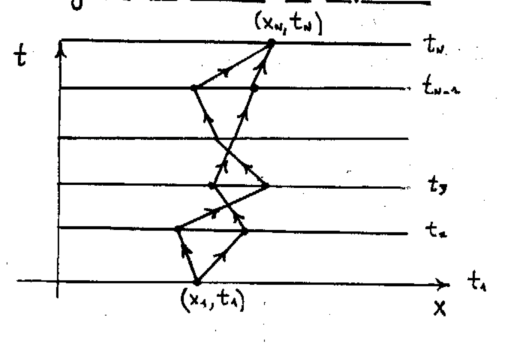
\includegraphics[width=0.6\textwidth]{images/teo2_8.pdf}	 
	\end{center}
	\caption{}
\end{figure} 

\[
	a
\]

Se puede pensar como que estamos sumando sobre todos los posibles caminos entre $(x_1,t_1)$ y $(x_N,t_N)$ 
fijos. En mecánica clásica teníamos un solo camino, el que minimizaba la acción $S$
\[
	\delta \int_{t_1}^{t_2} \Lag dt = \delta S = 0
\]
pero en cambio en mecánica cuántica todos los caminos aportan. En un libro de Dirac, Feymann lee 
\[
	a
\]
Definiremos
\[
	\equiv 
\]
Luego para considerar la suma sobre todos los segmentillos a lo largo de un camino tendremos
\[
	\prod_{n=2}^N \euler^{i/\hbar S(n,n-1)} =
\]
y hay que considerar TODOS los posibles caminos 
\[
	\propto \sum_{caminos} \euler^{i/\hbar S(N,1)} 
\]
cuando $\hbar \to 0$ las trayectorias contribuyen con una cantidad que oscila loca y violentamente. Tienden a 
la cancelación para caminos aledaños. Por el $\hbar \sim 0$ la fase es grande y entonces se cancelan.
Esto no ocurre cerca del camino (real) que cumple 
\[
	\delta S(N,1) = 0
\]
Para trayectorias cercanas la $\Delta fase$ no es grande y hay interferencia constructiva.
Para un $\delta t$ infinitesimal es 
\[
	a
\]
\[
	b
\]

\begin{figure}[htb]
	\begin{center}
	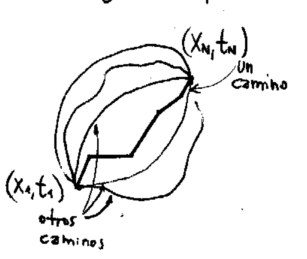
\includegraphics[width=0.6\textwidth]{images/teo2_9.pdf}
	\end{center}
	\caption{}
\end{figure} 

Consideremos, por ejemplo, una partícula libre, entonces $V=0$ de modo que resolviendo 
\[
	a
\]
Esto no es otra cosa que el propagador de una partícula libre. Para un $\Delta t$ finito será 
\[
	+
\]
\[
	=
\]
siendo esta última la integral de camino de Feynmann.

En base a éstas Feynamn desarrolla una formulación equivalente de la mecánica cuántica que utiliza los 
conceptos de:
\begin{enumerate}
 \item Superposición
 \item Composición de la transición
 \item Límite clásico con $\hbar \to 0$
\end{enumerate}

Estas integrales contienen toda la información del sistema cuántico, aunque no sea sencillo extraerla.

Consideremos un propagador de $(x',0) \to (x',t)$
\[
	G(t) =
\]
\[
	G(t) =
\]
y tomando Laplace-Fourier 
\[
	\tilde{G}(t)
\]

La expresión 
\[
	\equiv Integral de camino de Feynmann
\]
satisface la ecuación de Schrödinger y es una alternativa a la formulación de la cuántica usual.

% =================================================================================================
\section{Introducción al momento angular (rotaciones)}
% =================================================================================================

El operador $\hat{L}$ será el encargado de realizar las rotaciones. Por el álgebra visto en la mecánica 
clásica sabemos que, dado un vector \vb{v} y una matriz ortogonal $R$ se tiene
\[
	\vb{v}' = R \vb{v} \qquad \text{con} \quad |\vb{v}'|=|\vb{v}|
\]
y 
\[
	|\vb{v}|^2 = V^t V = (V^t R^t) (R V) \qquad \text{pues} \quad R^tR=RR^t = \mathbb{1}
\]
puesto que es una matriz ortogonal. Luego se cumplen 
\[
	clausura	
\]
el producto de dos matrices ortogonales es otra matriz ortogonal
\[
	asociatividad
\]
\[
	E identidad
\]
\[
	E inversa
\]

\subsection{No conmutatividad de las rotaciones clásicas}

Las rotaciones finitas no conmutan. Luego, el grupo de las rotaciones será un grupo abeliano
\[
	R_z(\varphi) = \begin{pmatrix}
	 \\
	\end{pmatrix}
\]
\[
	R_x(\varphi) = \begin{pmatrix}
	 \\
	\end{pmatrix}
\]
\[
	R_y(\varphi) = \begin{pmatrix}
	 \\
	\end{pmatrix}
\]

\begin{figure}[htb]
	\begin{center}
	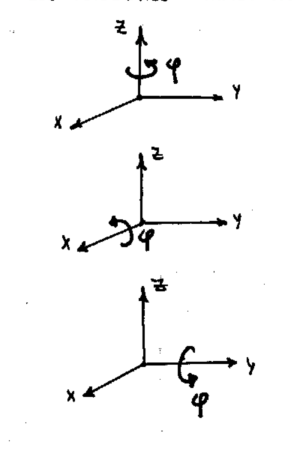
\includegraphics[width=0.6\textwidth]{images/teo2_10.pdf}
	\end{center}
	\caption{}
\end{figure} 

Si reemplazamos $\cos(\epsilon) \approx 1 - \epsilon^2/2$ y $\sin(\epsilon) \approx \epsilon$ hasta orden dos.
Se puede ver que las rotaciones, en torno a ejes diferentes, sólo conmutan a orden uno $(\epsilon)$ de manera 
que una rotación infinitesimal $d\varphi$ conmuta pero una rotación finita $\varphi$ no lo hace.

% =================================================================================================
\section{Rotaciones cuánticas}
% =================================================================================================

Para las rotaciones cuánticas se pedirá
\[
	D,
\]
rotación infinitesimal o bien
\[
	D,
\]
para rotación finita. Donde $\hat{D}$ es el operador de las rotaciones y $\hat{J}$ es un momento angular 
general. Se postula de esta forma para que $\hat{D}$ cumpla las mismas propiedades que $R$ y la relación de 
conmutación
\[
	R_x R_y - R_y R_x = R_z (\epsilon^2) - \mathbb{1}
\]
\[
	D
\]
de modo que la cuenta lleva a  
\[
	J_x
\]
la cual generalizando se llega a 
\[
	[J_i,J_j] = i \hbar \epsilon_{ijk} J_k
\]
que son las relaciones de conmutación generales para momento angular $\hat{J}$.

Para sistemas de spín $1/2$ es 
\[
	D(\hat{n},\phi) \equiv \euler^{-i/\hbar \vb{S}\cdot\hat{n} }
\]
Se puede ver que ante rotaciones cuánticas $D(\hat{n},\phi)$ los valores de expectación transforman como 
vectores
\[
	=
\]

En general $\vb{J} = (J_x, J_y, J_z)$ se transforma como vector y entonces $\hat{J}$ es un operador vectorial.
Para spín $1/2$ es
\[
	\Ket{alpha} =
\]
\[
	D
\]
\[
	D
\]
Si $\phi=2\pi$ (cosa que debiera dejar al ket incólume) se tiene 
\[
	D
\]

Luego, esto es una muestra del carácter no-clásico del spin; una vuelta completa le cambia el signo al ket 
pero notemos cuidadosamente que el valor de expectación -- que es algo físico -- no varía. Esto muestra que 
el ket no puede tener sentido físico.

\subsection{Angulos de Euler}

Se define una serie de rotaciones 
\[
	1 2 3
\]
lo cual equivale a
\[
	R() = 
\]
\[
	\euler
\]

Pero desconozco cómo operar en los ejes móviles $z',y'$
\[
	R_{y'}(\beta) =
\]
\[
	R_{z'}(\gamma) =
\]
\[
	R() =
\]
Rotación equivalente a [1] pero para ejes fijos, puesto que en mecánica cuántica sabemos rotar en torno a 
ejes fijos.

Los ángulos de Euler son la caracterización de una rotación general en 3D.

Entonces nuestra rotación en 3D cuántica será:
\[
	D() =
\]

\subsection{Autoestados y autovalores de J}

Partimos de 
\[
	[] = 
\]
y
\[
	J^2 = , [J^2,J] = 0
\]
siendo la última muy importante y probándose por evaluación directa. Lleva a 
\[
	[J^2,J_i^n] = 0 \qquad \text{con} \; i=x,y,z \; n\in\mathbb{N}
\]

Se eligen $J^2, J_z$ como observables que conmutan 
\[
	J^2
\]

Definiremos los operadores de subida y de bajada
\[
	J_{\pm} \equiv J_x \pm J_y
\]
que verifican 
\[
	[]
\]
Entonces se tiene 
\[
	J^2() \longrightarrow 
\]
\[
	(J_z) \longrightarrow
\]

\[
	J_{\pm} \Ket{a,b} = C_{\pm} \Ket{a,b\pm\hbar}
\]
\[
	J_+
\]
sube el $J_z$ en una unidad de $\hbar$ o bien baja el $J_z$ en una unidad de $\hbar$.
\[
	J_+J_- =  ,
\]
\[
	J^2 = ,  
\]
\[
	\Braket{a,b|J^2 - J^2_z|a,b} = 
\]
\[
	(a-b^2)\Braket{a,b|a,b} = , a \geq b^2
\]
hay cota para $b$.
Como no puede seguir subiendo debe dar el ket nulo 
\[
	= 0
\]
\[
	= 0
\]
pero 
\[
	J_-J_+
\]
\[
	= 0	\qquad a = b_m(b_m-\hbar)
\]
tiene solución 
\[
	b_M - B_m = - \hbar
\]
pero esto es absurdo.

Luego,
\[
	\Ket{a,b_m} \longrightarrow \Ket{a,b_M}
\]
y como $J_+$ sube de a un $\hbar$ será
\[
	b_M = b_m + n\hbar
\]
y entonces
\[
	b_M = \frac{n\hbar}{2} = \frac{n}{2} \hbar = j \hbar
\]
y se da que $j$ es entero o semientero.

Definiremos 
\[
	b_M \equiv j \hbar \qquad a \equiv j (j+1) \hbar^2 \qquad -j\hbar \leq b \leq j\hbar
\]
pero como $b/\hbar = m$
\[
	b_M \equiv j \hbar \qquad a \equiv j (j+1) \hbar^2 \qquad -j \leq m \leq j
\]
\[
	m = (-j,-j+1,-j+2,...,j-1,j) \qquad 2j+1 \text{valores de} \; m
\]
\[
	J^2 \Ket{j,m} = j( j+1 )\hbar^2\Ket{j,m} \qquad J_z \Ket{j,m} = m \hbar \Ket{j,m}
\]

\subsection{La normalización de $J_\pm$}

\[
	J_+
\]
\[
	\Braket{j,m|J_-J_+|j,m} = 
\]
\[
	c_+ = 
\]
\[
	\Braket{j,m|J_+J_-|j,m} = 
\]
\[
	c_- =
\]
\[
	J_+
\]

\subsection{Elementos de matriz de $J^2, J_z, J_+$}

Asumiendo normalización de $\Ket{j,m}$ se tiene 
\[
	\Braket{} = 
\]
\[
	=
\]

\subsection{Elementos de matriz de $\mathcal{D}(R)$}

Ahora queremos ver cual es la forma de los elementos de matriz de $\mathcal{D}(R)$
\[
	\mathcal{D}(R) =
\]
siendo que $\mathcal{D}(R)$ tiene por efecto rotar el sistema físico.
Lo primero que hay que notar es que 
\[
	\propto \delta_{jj'}
\]
porque $[J^2,J_i]=0$ y entonces $[J^2,J_i^n]=0$ y 
\[
	D
\]
y 
\[
	D
\]
es una matriz para cada $j$ fijo con $\{ (2j+1)\times(2j+1)=\text{dimensión}\}$
\[
	D
\]
pero las rotaciones no cambian el $j$, $\mathcal{D}(R)$ conecta estados con la misma $j$ y $\mathcal{D}(R) 
\in (2j+1)\times(2j+1)$ 
\[
	D
\]

La matriz de $\mathcal{D}(R)$ (no caracterizada por un único $j$) puede ponerse en forma diagonal por bloques:


con cada bloque de $(2j+1)\times(2j+1)$ , pero siendo cada bloque irreducible. Las matrices de rotación con 
$j$ fijo forman un grupo. $\mathcal{D}_{m'm}^{(j)}(R)$ son los elementillos de la matriz.
\[
	\Ket{j,m} \longrightarrow
\]

\subsection{Forma explícita del operador $\mathcal{D}(R)$}

Los ángulos de Euler permitieron caracterizar la rotación más general. Entonces 
\[
	D
\]
\[
	D
\]

En los $d_{m'm}^{(j)}$ está la dificultad de la cuenta.

% =================================================================================================
\section{Formalismo de spinores de Pauli}
% =================================================================================================

Apropiado para trabajar con sistemas de spín $1/2$. Estos sistemas son casos particulares de momento angular,
\[
	j = 1/2 \qquad m=-\frac{1}{2},+\frac{1}{2}
\]
y se definen los spinores $\chi_\pm$ como
\[
	\Ket{+} \equiv  \begin{pmatrix}
	                 1 \\ 0 
	                \end{pmatrix} \equiv  \chi_+
\]

Para spín $1/2$ podemos tomar $\vb{J} = \vb{S}$ por la analogía de las relaciones de conmutación.
A su vez 
\[
	\vb{S} = \frac{\hbar}{2} \vec{\sigma} \; \text{con} \;
\]
que es una especie de vector 
\[
	\sigma
\]
Luego esta equivalencia provee expresión de los operadores $S_i$ en términos de matrices de $2\times 2$, así:
\[
	\frac{i}{2}[ J_- - J_+] = J_y = S_y = \frac{\hbar}{2} \sigma_y
\]

Las matrices de Pauli cumplen las propiedades básicas siguientes 
\[
	\sigma^2_i = \mathbb{1}
\]
\[
	\Ket{+} \qquad (\sigma\dot\vb{a})
\]

\subsection{Aplicación a las rotaciones}

\[
	D
\]
pero 
\[
	()^n= 
\]
\[
	\euler
\]
\[
	d
\]
es el operador de rotación para sistemas de spin $1/2$. Con esta expresión podemos evaluar 
$d^{j=1/2}_{m'm}(\beta)$
\[
	d
\]
donde hemos usado los resultados 
\[
	\cos \sin 
\]

En el caso general el operador de rotación para sistemas de spin $1/2$ lucirá:
\[
	D = 
\]

\subsection{Ejemplo}

\[
	d
\]
Este resultado es intuitivamente lógico.


\subsection{Rotaciones en sistemas con $j=1$}

Ahora tenemos 
\[
	j=1 \qquad m = -1,0,1
\]
recordando $J_y$ en términos de escaleras
\[
	J_y
\]
\[
	\euler
\]
\[
	\left( \frac{J_y}{\hbar} \right)^n =
\]
\[
	\euler =
\]
acá lo vemos como operador (es notación), $d_{m'm}^{j=1}(\beta)$ simboliza la matriz
\[
	d
\]

% =================================================================================================
\section{Momento angular orbital}
% =================================================================================================

\[
	\vb{L} =
\]
verifica el álgebra de $\vb{J}$,
\[
	[]
\]
Consideremos ahora una rotación en torno a $z$, en un $\delta\phi$,
\[
	() =
\]
\[
	() = 
\]
esto es una traslación en $\hat{x},\hat{y}$,
\[
	(1-i\frac{L_z}{\hbar}\delta\phi) \Ket{x',y',z'} = \Ket{}
\]

Esta traslación es debida a una rotación infinitesimal en $\delta\phi$ torno a $z$ entonces genera las 
rotaciones clásicas en torno a $z$.
\[
	\Psi 
\]
\[
	\Psi
\]

Podemos hallar una expresión para $L_z$ en esféricas:
\[
	\Braket{r,\theta,\varphi||\alpha}
\]
identificamos 
\[
	= 
\]
operador $L_z$ en esféricas

Usando 
\[
	L^2 = 
\]
\[
	\Braket{L^2}
\]
\[
	L^2 = -\hbar^2 r^2 \nabla^2_{\theta,\varphi}
\]
donde $\nabla^2_{\theta,\varphi}$ es la parte angular del laplaciano en coordenadas esféricas.
Esto puede obtenerse también partiendo de 
\[
	L^2 = \vb{x}^2\vb{p}^2 - (\vb{x}\cdot\vb{p})^2 + i\hbar \vb{x}\cdot\vb{p}
\]

Sea un $H$ de partícula, sin spín, sujeta a potencial simétricamente esférico. Sabemos que la función de onda 
$\Psi_\alpha(\vb{r}')$ es separable en coordenadas esféricas, entonces:
\[
	\Braket{|} = 
\]
\[
	\Braket{|} = 
\]

Cuando el H es esféricamente simétrico (como en un potencial central) se tiene 
\[
	[] = [] = 0
\]

Trabajaremos solamente en la parte angular  $\Ket{\theta,\varphi} \equiv \Ket{\hat{n}}$
\[
	\Braket{\hat{n}|\ell,m} =
\]
que es la amplitud de hallar $\Ket{\ell,m}$ en la dirección $\hat{n}$.

Podemos vincular ahora los armónicos esféricos con los autoestados de $L_z,L^2$
\[
	L_z
\]
\[
	L^2
\]
\[
	=
\]
Entonces, con la ortogonalidad
\[
	\longrightarrow
\]
y con la completitud 
\[
	\longrightarrow
\]
de manera que llegamos a 
\[
	\int \int 
\]

Podemos hallar una expresión para 
\[
	= 0
\]
\[
	\Rightarrow
\]

Luego usamos $L_-$ para hallar sucesivamente los demás $Y^m_\ell$
\[
	=
\]
y por este camino se llega a 
\[
	Y
\]
con 
\[
	\qquad 
\]

En el caso de momento angular orbital $\ell$ no puede ser semientero porque entonces $m$ sería semientero y 
en una vuelta de $2\pi$
\[
	\euler^{im2\pi} = -1
\]	

Además,
\[
	\text{(no hay signo menos)}
\]

\subsection{Armónicos esféricos como matrices de rotación}

Se pueden hallar autoestados de dirección $\Ket{\hat{n}}$ rotando el $\Ket{\hat{z}}$,
\[
	\hat{n} = 
\]
Necesitamos aplicar 
\[
	D
\]
\[
	n
\]
\[
	l
\]
\[
	l
\]
\[
	Y
\]
pero como $\theta=0$ , $Y_\ell^m = 0$  con $m\neq 0$ se tiene 
\[
	lm
\]
\[
	Y^*,
\]
la matriz de rotación en este caso es un armónico esférico.

La $\Psi$ tiene la misma simetría que el potencial.

% =================================================================================================
\section{Suma de momentos angulares}
% =================================================================================================

\subsection{Dos momentos de spín $1/2$}

Sean dos estados de spín $1/2$
\[
	a
\]
en cada espacio valen las relaciones usuales de conmutación 
\[
	b, [S_{1i},S_{2j}] = 0
\]
donde el último indica que operadores de espacios diferentes conmutan.

Un estado general es 
\[
	a
\]
Hay cuatro estados
\[
	b
\]
que corresponden a los operadores $S_ 1^2, S_2^2, S_{1z}, S_{2z}$ que conmutan (son un CCOC).

Podemos elegir otras base de operadores que comutan que será: $S_ 1^2, S_2^2, S, S_{z}$, de modo que el estado general 
será
\[
	c
\]
Así tendremos
\[
	d
\]
\[
	S 2 =  \qquad 
\]

Dada la repetición de $S_1,D_2$ se suelen identificar a las bases solamente 
\[
	d
\]
Además la base $\{ \Braket{m_1,m_2}\}$ se puede poner como 
\[
	+ \equiv + 1/2 \qquad\qquad - \equiv - 1/2
\]

\subsection{Cambio entre bases}

Podemos hallar a ojo que 
\[
	\cdot \Ket{++} = \Ket{1,1} \qquad \cdot \Ket{--} = \Ket{1,-1} 
\]
de manera que la única forma de tener $m=1$ es con los dos spines up y la única forma de tener $m=-1$ es con los dos 
spines down.

Se hallan los otros con el operador de bajada
\[
	S_- \equiv S_{1-} + S_{2-}
\]
y si descompongo $S_-$ en $S_{1-}$ y $S_{2-}$ para operar en $\Braket{s,m}$ se tiene 
\[
	S
\]
y ahora si opero con $S_-$,
\[
	S
\]

Luego
\[
	\Braket{00}
\]
y puedo usar ortonormalidad 
\[
	= 0 = \qquad \text{con} \; |a|^2 + |b|^2 = 1
\]
\[
	\cdot 
\]


\section{Teoría formal de suma de momentos angulares}

Sea de sumar dos momentos angulares $J_1, J_2$. Las relaciones de conmutación son
\[
	[] = i\hbar \varepsilon_{ijk}J_{1k} \qquad [] = i\hbar \varepsilon_{ijk}J_{2k} \qquad
	[J_{1k},J_{2k}] = 0
\]
\[
	\vb{J} = \otimes + \otimes \equiv \vb{J}_1
\]
\[
	[]
\]

El momento total \vb{J} cumple que 
\[
	J^2 = 
\]
donde vemos que 
\[
	[] =
\]
pero 
\[
	[ J^2 , J_{1z}] \neq 0  \qquad \qquad [ J^2 , J_{2z}] \neq 0
\]

Esto deja dos opciones para elegir un CCOC

\begin{center}
\begin{tabular}{|c|c|}
\hline 
$J_1^2, J_2^2, J_{1z}, J_{2z}$ & $J_1^2, J_2^2, J^2, J_{z}$ \\
$\Ket{j_1,j_2;m_1,m_2}$ & $\Ket{j_1,j_2;j,m}$ \\
base desacoplada & base acoplada \\
\hline
\end{tabular}
\end{center}



Se puede pasar de uan base a otra con una identidad $\mathbb{1}$ apropiada
\[
	\Ket{j_1,j_2;j,m} =
\]
\[
	1.
\]
\[
	a
\]
\[
	2.
\]
\[
	a
\]

Donde los $C_{m_1 m_2}^j$ son los coeficientes de Clebsh-Gordan. En 2 la $\sum$ sería en $j\to\infty$, pero veamos la 
relacion que hace algunos $C_{m_1 m_2}^j=0$. Ante todo abreviaremos suprimiendo los índices $j_1,j_2$ con lo cual 
\[
	C
\]

\subsection{Restricciones para la no nulidad de los coeficientes}

\[
	a
\]
\[
	b
\]
\[
	\Braket{m_1,m_2| j,m} \neq 0 \Rightarrow m = m_1 + m_2
\]

A su vez, en la suma de $J_1$ y $J_2$ resultan los $j$ acotados por una desigualdad triangular 
\[
	|| \leq j \leq j_1 + j_2
\]

Asimismo los $C_{m_1 m_2}^j$ se toman reales, entonces 
\[
	C
\]
y juntando todo se tiene 
\[
	\Rightarrow
\]

Ambas bases tienen la misma dimensión
\[
	\sum = (2j_1 + 1)(2j_2 + 1)
\]

Recordemos que cada $j$ tiene $2j+1$ estados posibles (los $m$ correspondientes a cada $j$) ($|m|\leq j$). Si sumamos 
$j_1=1, j_2=3/2$ tendremos 
\[
	dim
\]
\[
	j = 1/2, 3/2, 5/2
\]

Podemos ver a ojo que 
\[
	\Ket{j}
\]
luego con el $J_=, J_-$ podemos construirnos los siguientes (utilizando ortonormalidad)
\[
	= 
\]
\[
	= \qquad \sum = 1
\]

\subsection{Relación de recurrencia}

\[
	J_\pm = \ ket{j,m} = 
\]
\[
	b
\]
y metiendo un bra $\Bra{m_1,m_2}$ se llega a la relación de recurrencia
\[
	\sqrt{()}
\]

\subsection{Suma de \vb{L} y \vb{S}}

Sea suma \vb{L} y \vb{S}, entonces 
\[
	a
\]
habrá sólo cuatro $C_{m_1 m_2}^j$ no nulos, que serán 
\[
	\Braket{|}
\]
donde vemos que los coeficientes linkean sólo los estados con $j=\ell-1/2$ y $j=\ell+1/2$ y podemos construir una 
matriz de $2\times 2$ para este caso.

Esto tórnase práctico para acoplamiento spin-órbita 
\[
	LS
\]
\[
	LS
\]
\[
	LS
\]

\section{Operadores vectoriales}

Queremos analizar como transforma un operador vectorial $\hat{v}$ bajo rotaciones en mecánica cuántica.
En mecánica clásica,
\[
	V_i = R_{ij} V_j \qquad \text{con} \; R \; \text{matriz diagonal}
\]
En mecánica cuántica tenemos que al rotar
\[
	=
\]
Pediremos entonces que $\Braket{V}$ transforme como un vector y eso lleva a que 
\[
	=
\]
\[
	\mathcal{D}(R)^+
\]
y calculando la expresión anterior 1 llegamos a que debe valer
\[
	[V_i,J_j] =  i\hbar \varepsilon_{ijR}V_R
\]
que es la manera de transformar de un operador vectorial. Podemos probar un caso simple de una rotación infinitesimal 
en $\hat{z}$ y ver que vale.


\section{Operadores tensoriales}

En mecánica clásica 
\[
	T_{ij} 
\]
que es un tensor de rango dos. Esto es un tensor cartesiano. Su problema es que no es irreducible, entonces puede 
descomponerse en objetos que transforman diferente ante rotaciones. Sea la díada $U_iV_j$, tensor de rango dos, que 
puede escribirse como 
\[
	UV =
\]
Hemos reducido el tensor cartesiano en tensores irreducibles. Podemos asociar esta descomposición con las 
multiplicidades de objetos con momento angular $\ell=0, \ell=1, \ell=2$
\[
	\text{escalar} \longrightarrow \ell=0 \; \text{singlete (un elemento independiente) }
\]
\[
	\text{vector} \longrightarrow \ell=1 \; \text{triplete (tres elementos independientes)}
\]
\[
	\text{tensor de traza nula} \longrightarrow \ell=2 \; \text{quintuplete (cinco elementos 
independientes)}
\]

Se define 
\[
	T^{(k)}_q \qquad \text{tensor esférico de rango $k$ y número magnético $q$}
\]
Un tensor esférico transforma como 
\[
	D T D = D T 
\]
Tendremos 
\[
	T^{(0)}_0 \quad \text{(escalar) tensor esférico de rango 0 ($\ell=0$)}
\]
\[
	(T^{(1)}_1,T^{(1)}_0,T^{(1)}_{-1}) \quad \text{(vector) tensor esférico de rango 1 ($\ell=1$)}
\]

En muchos casos se puede escribir un tensor esférico como armónico esférico 
\[
	Y_\ell^{m}(\theta,\varphi) = Y_\ell^{m}(\hat{n})  \overbrace{\hat{n} \longrightarrow 
	\vec{v}}^{\text{paso}} Y_\ell^m(\vec{v}) \equiv Y_k^q(\vec{v}) = T_q^{(k)}
\]
\[
	\hat{n} = ()
\]
\[
	Y \longrightarrow T
\]
\[
	Y
\]
Calculando en 2, cosa que podemos hacer para, por ejemplo, una rotación infinitesimal, llegamos a las 
relaciones de conmutación para tensores.
\[
	[]
\]


\section{Teorema de Wigner-Eckart}

Es importante para el cálculo de transiciones evaluar elementos de matriz de operadores tensoriales.
Los elementos matriciales de operadores tensoriales respecto de autoestados de momento satisfacen 
\[
	\Braket{||} =
\]
un coeficiente que no depende de $q,m,m'$.

La regla de selección se construye 
\[
	\Braket{[]} =
\]
\[
	\neq
\]

Una idea de la demostración del teorema
\[
	sa
\]
\[
	ba
\]

Es la misma relación de recurrencia que la de los coeficientes de Clebsh-Gordan, si reemplazamos
\[
	m'=m \quad j=j_1 \quad m=m_1 \qquad j'=j \quad k=j_2 \quad q=m_2
\]

Como ambas relaciones son lineales, sus resultados serán proporcionales.
Se puede asociar 
\[
	\propto 
\]
\[
	\propto
\]
Logramos la igualdad metiendo una constante independiente de $m',q,m$.

\subsection{Reglas de selección}

Como se tiene a $\Braket{|T_q^{(k)}|}$ proporcional a los coeficientes de Clebsh-Gordan, serán válidas las 
mismas reglas de selección 
\[
	m' = m + q \qquad |j-k| \leq j' \leq j+k
\]

\section{Ejemplos de elementos matriciales de tensores}

Sea un escalar (tensor de rango cero)
\[
	\Braket{||} =
\]

No varían $j,m$ en los estados No conecta estados con $j,m$ diferentes un escalar.

Sea un vector (tensor de rango uno):
\[
	\Braket{||} \propto \Braket{j 1;m q|j 1;j' m'}
\]

Conecta estados que están separados por un $j$ y un $m$.

\subsection{Teorema de proyección}

Consideremos lo que sucede en el teorema de Wigner-Eckart si $j=j'$ y se lo aplicamos a un operador vectorial 
$T_q^{(k=1)} \equiv V_q$
\[
	=
\]

Como caso especial, si $\alpha' =\alpha$ estoy en un subespcaio donde coinciden los números cuánticos, se 
tiene
\[
	\vb{V} = \frac{\Braket{\cdot}}{} \vb{J}
\]

\subsection{Aplicación del teorema de proyección}

Sea un $H_0$ esféricamente simétrico 
\[
	cosas
\]

Si meto un campo $B$ en $\hat{z}$ tendré 
\[
	H \equiv H_0 + H_1 = H_0
\]
lo cual debería romper la degeneración.
\[
	L_z + 2S_z =
\]
pero no puedo poner este nuevo operador, que mete el campo B, en el CCOC directamente, entonces uso teorema 
de proyección.
\[
	escalares
\]
Entonces tengo todo expresado en función de $J_z$ que sí forma parte de mi CCOC.


\section{Simetrías en mecánica cuántica}

En mecánica clásica tenemos el teorema de Noether 
\[
	\partial p_i = cte.
\]
Y $\mathcal{H}, \mathcal{L}$ no cambian con la transformación $q_i \longrightarrow q_i + \delta q_i$
\[
	\partial 
\]

En mecánica cuántica definiremos un operador unitario $\$$ asociado a traslación/rotación. Pensemos en una 
transformación infinitesimal dada por $\$$
\[
	\$
\]

Sea el H invariante frente a $\$$, entonces 
\[
	SHS =
\]

Esto significa que el autovalor no varía con el tiempo, Como $[H,G]=0$ se tiene 
\[
	no dege 
\]

\subsection{Simetría de paridad}

Transforma un RHS en LHS. Es decir que hace 
\[
	\vb{x} \longrightarrow - \vb{x}
\]
y solicitaremos un operador unitario llamado paridad que verifique 
\[
	\Ket{\alpha} \longrightarrow \Pi\Ket{\alpha} = \Ket{\alpha'}
\]
si $\Pi$ es unitario y $\Pi^1=\mathbb{1}$ entonces es hermítico.
Queremos que refleje el $\Braket{\hat{x}}$ 
\[
	a
\]
anticonmuta con \vb{x}.
Debido a ello 
\[
	a
\]
como $\hat{\Pi}$ no depende del tiempo 
\[
	d
\]
y vemos que anticonmuta con \vb{p}.
\vb{x}, \vb{p} son operadores impares. En cambio $\vb{L}=\vb{x}\times\vb{p}$ es un operador par, entonces 
\[
	[] = 0
\]

Que conmuta con \vb{J} puede verse de pedirle que 
\[
	[] = 0 \longrightarrow [] = 0 ,
\]
cosa que vale en mecánica clásica, entonces 
\[
	R
\]
\[
	\Box
\]
\[
	\Box
\]

\subsection{Función de onda bajo paridad}

\[
	\Psi
\]
y entonces la función de onda de un estado al que se le aplicó paridad será 
\[
	\Psi
\]

Sea $\Ket{\alpha}$ autoestado de paridad, entonces 
\[
	a
\]
los autovalores serán $\pm 1$
\[
	=
\]
no toda función de onda tiene paridad bien definida.

\[
	\vb{x}
\]
\[
	=
\]
\[
	\Pi
\]
Como $[\vb{L},\hat{\Pi}]=0$ un autoestado de \vb{L} es autoestado de $\hat{\Pi}$ .

\subsection{Teorema}

Sea 
\[
	autoestado 
\]

La demostración 
\[
	()
\]
\[
	2
\]
\[
	3
\]

Un caso donde falla el teorema 
\[
	caso
\]
\[
	caso mas
\]

\subsection{Reglas de selección de paridad $\Pi$}

Sean $\Ket{\alpha}, \Ket{\beta}$ autoestados de paridad 
\[
	\Pi
\]
\[
	\Braket{||}
\]

\begin{itemize}
 \item Operadores impares solo conectan estados de paridad opuesta
 \[
	a
 \]
 \item Operadores pares solo conectan estados de la misma paridad 
 \[
	b
 \]
\end{itemize}

\[
	= 0
\]
\[
	c
\]

\section{Inversión temporal (reversión de movimiento)}

En mecánica clásica sería {\it pasar la película hacia atrás}
\[
	t \longrightarrow -t
\]
En sistemas sin fuerzas disipativas se tiene 
\[
	m \ddot{x} =
\]

En mecánica cuántica tendremos 
\[
	i \hbar 
\]
\[
	=
\]
no es solución de Schrödinger. 
Pero notemos que $\Psi^*(x,-t)$ cumple la ecuación de Schrödinger
\[
	i\hbar
\]

Entonces necesitamos un operador que respete esta característica. Necesitaré el producto interno conjugado 
\[
	\Psi
\]
El operador involucrado no será unitario 
\[
	\Ket{\tilde{\alpha}} = 
\]
Si $\hat{\Theta}$ unitario se conserva el producto interno 
\[
	=
\]

Pediremos antiunitariedad y antilinealidad al operador $\hat{\Theta}$
\[
	=
\]
\[
	=
\]

Todo operador antiunitario y antilineal puede escribirse como producto 
\[
	\Theta = U K
\]
donde $U$ es unitario y $K$ la conjugación compleja. $K$ no cambia los autoestados, porque en base canónica 
un autoestado tiene un solo elemento (1) que no es nulo.
\[
	K
\]

Veamos que $UK$ es antiunitario 
\[
	=
\]

\[
	=
\]
\[
	=
\]

Notemos que no se define $\hat{\Theta}^\dagger$ actuando sobre bras. La demostración anterior esperó a 
quitarse de encima $\hat{K}$ para hacer dual conjugado al $\Ket{\tilde{\beta}}$.

\subsection{Operadores ante $\hat{\Theta}$}

Usaremos la notación 
\[
	\Ket{\tilde{\alpha}} = \hat{\Theta} \Ket{\alpha}
\]
donde hay que tener en cuenta 
\[
	= \mathbb{1}
\]

Sería razonable esperar que 
\[
	= -
\]
Sea $\hat{\mathbb{O}}$ un operador hermítico 
\[
	=
\]
Luego metemos un $=1$
\[
	=
\]

Notamos que no se aplica $\Theta$ sobre bra alguno y tenemos $\Theta$ no unitario. Entonces requeriremos 
\[
	=
\]
como para $\vb{p},\vb{J}$ operadores impares 
\[
	=
\]
y $\vb{x}$ operador par.

Los operadores pares conmutan con $\Theta$,
\[
	= =
\]

Hamiltoniano ante reversión de movimiento. Veamos la reversión de un sistema en estado $\Ket{\alpha}$
\[
	=
\]
Si el hamiltoniano es invariante ante reversión temporal debería ser lo mismo 
\[
	=
\]
es decir que estamos pidiendo que se obtenga el mismo estado 
\begin{itemize}
 \item Si revertimos el movimiento y evolucionamos $\delta t$.
 \item Si evolucionamos hacia atrás $-\delta t$ y revertimos el movimiento.
\end{itemize}

Veamos que vale lo anterior, pensando que si vale se tiene 
\[
	=
\]
\[
	=  \qquad [H,\Theta]=0
\]

Si $\Theta$ era unitario teníamos la relación de anticonmutación $\{ H, \Theta \}=0$ lo cual lleva a absurdos.
\[
	a
\]
Si $\{ H,\Theta \} = 0$
\[
	= \text{H debe ser par frente a $\Theta$}
\]

\subsection{Función de onda}

Sea en $t=0$ un sistema en el estado $\Ket{\alpha}$
\[
	= = 
\]
\[
	\Psi
\]
Esto era lo que {\it vimos} en la ecuación de Schrödinger.

\subsection{Reversión de movimiento sobre \vb{J}}


no tiene sentido porque $J_x,J_y,J_z$ no conmutan entre ellos. Analizaremos $\Ket{\ell,m}$
\[
	\Theta \Ket{\vb{J}} 
\]
\[
	\equiv 
\]

Lo que hace $\Theta$ es invertir la componente de $\hat{z}$ y alterar la fase. Se ve que 
\[
	\Theta^2 = \mathbb{1}
\]

\subsection{Reversión para sistemas de spin $1/2$}

Sea un estado general up de spin $\Ket{\hat{n};+}$, que se obtiene con dos rotaciones 
\[
	Sn
\]
\[
	\Theta
\]
\[
	a
\]
\[
	b
\]
\[
	c
\]

\subsection{Teorema}

Sea $H$ invariante ante $\Theta$ y los $\Ket{n}$ no degenerados, entonces la autofunción de energía puede 
hacerse real tomando una fase apropiada.

Demostración 
\[
	H \Theta  \Ket{n} =
\]
\[
	=
\]
\[
	=
\]

Si le aplico al sistema transformaciones dadas por operadores que conmutan con el H no lo sacamos del 
autoestado en que se encuentra con el paso del tiempo.
En ese sistema solo será razonable medir variables representadas por esos operadores; puesto que de lo 
contrario estamos alterando el sistema y nos es imposible saber donde ha quedado.

\section{Métodos perturbativos}

Se basan en 
\[
	H = H_0 + \lambda V \qquad \lambda \ll 1
\]
con $ H_0\Ket{n^{(0)}} = E_n^{(0)}\Ket{n^{(0)}}$ (el problema sin perturbar)
\[
	H
\]
que sería la solución exacta.
Como esto es hartocomplicado podemos desarrollar en serie 
\[
	\approx 
\]
\[
	\approx 
\]
\[
	()[] = ()()
\]
\[
	\sum_{i=0}^\infty =
\]
y aproximando los primeros términos 
\[
	H_0
\]
\[
	E_0
\]
ahora igualamos orden a orden y resulta 
\[
	\lambda^0 ....
\]
\[
	\lambda^1 ....
\]
\[
	\lambda^2 ....
\]

Pediremos una normalización a cada orden y considerando $ \Braket{0_n|n(\lambda)} \in \mathbb{R}$
\[
	()() =
\]
\[
	\lambda
\]
\[
	...
\]
\[
	...
\]

En un mismo autoestado $(n)$ los órdenes diferentes $(i)$ no son necesariamente ortogonales.

\section{Resolución}

A orden cero será 
\[
	() \qquad \text{y se define} \qquad 
\]
y $\Ket{0_n}$ es dato porque es el estado no perturbado.
A orden uno tenemos 
\[
	()
\]
\[
	\Braket{}
\]
y la energía a orden uno es 
\[
	=
\]

Veamos el autoestado a orden uno. Podemos poner (no hay degeneración)
\[
	=
\]
y sea $p\neq n$
\[
	+ = 0
\]
\[
	=
\]
a un mismo orden (cero) diferentes autoestados son ortogonales.
Sea $p=n$ entonces 
\[
	= 0 
\]
ya lo vimos antes, en la normalización
\[
	=
\]
autoestado hasta orden uno. A orden dos tenemos 
\[
	+ - = 0
\]
\[
	+ - = 0
\]
\[
	=
\]
\[
	E
\]
que es la energía a orden dos.
Veamos el autoestado a orden dos 
\[
	\Ket{2n} = \sum_p ()\Ket{\phi_p}
\]
sea $p\neq n$ 
\[
	+
\]
\[
	+
\]
\[
	=
\]
\[
	+
\]
\[
	+
\]

Sea $p=n$
\[
	+ = 1
\]
\[
	=
\]
\[
	=
\]

\[
	\Ket{2n} =
\]
y el autoestado hasta orden dos
\[
	=
\]
con la energía hasta orden dos 
\[
	=
\]

\subsection{Caso degenerado}

Sea que hay degeneración de orden $g$ en el autoestado $N$( a orden cero)
\[
	= k=1,2,...,g
\]
Suponemos existe combinación lineal 
\[
	+
\]
para escribir un estado degenerado en función de los otros.
\[
	= 0
\]
\[
	= 0
\]
\[
	=0
\]
\[
	=0
\]
\[
	=
\]
Esto último es una ecuación de autovalores y autovectores de la forma:
\[
	= 0 
\]
nos dará los corrimientos de la energía a primer orden  y los autoestados $\Ket{1_n^j}$ serán los 
autovectores del problema.

\section{Efecto Stark}

Sea un átomo de H con $\Ket{n,\ell,m}$ sin spín y con $n=2$. Será 
\[
	0
\]
Tengo cuatro estados 
\[
	2 0 0 
\]
todos con la misma energía $\epsilon_2$.
Metemos un campo eléctrico en $\hat{z}$ y entonces $V=-ez|\vb{E}|$. Luego 
\[
	=
\]
$\hat{z}$ es impar ante paridad y entonces vincula estados de paridad diferente,
y entonces 
\[
	= 0 
\]
diagonal nula y con $m'\neq m$ a igual $\ell$ tiene la misma paridad
\[
	=
\]

Solo hay un elemento no nulo correspondiente al producto par-impar.
Se tendrá 
\[
	=
\]
Puedo diagonalizar y obtengo 
\[
	=
\]

En este caso no se rompe la degeneración por completo.
\[
	=
\]


\subsection{Corrimiento de la energía a orden 2 (con degeneración)}

Sea que a orden uno se rompe toda la degeneración 
\[
	+ - = 0
\]
Entonces la corrección a segundo orden de la energía será:
\[
	+ - = E
\]
pues $\Braket{0_N^j|0_N^j}= 0$ pero 
\[
	=
\]
\[
	=
\]
falta desarrollo ...

\[
	E =
\]
donde $N$ es un estado degenerado.

\section{Estructura fina del átomo de hidrógeno}

La solución tradicional del átomo de H usa el potencial coulombiano. Esto desemboca en las funciones 
$\Ket{n,\ell,m}$, sin embargo la introducción de ajuste como {\it perturbaciones} rompe algo la degeneración.
\[
	cuentitas
\]
donde $a_0$ es el radio de Bohr, $\alpha$ es la constante de estructura fina .
Tenemos 
a) Corrección cinemática (relativista)
\[	
	0
\]
y esta corrección va como $W_{mv}/H_0 \sim \alpha^2$.

b) Acoplamiento spín-órbita
Se puede pensar considerando un $e^-$ en reposo con un protón orbitando que genera un $\vb{B}_{eff}$
\[
	W_{so} =
\]
y la corrección va como $W_{mv}/H_0 \approx \alpha^2$.

c) Término de Darwin o de contacto
\[
	=
\]
que va como  $W_{D}/H_0 \approx \alpha^2$.

Hay otras correcciones hiperfinas que provienen del spín del electrón y del spín del protón. Pero van como 
$\alpha^2/2000$.
Si consideramos el sistema con 
\[
	n=2
\]
serán ocho estados.
\[
	W
\]
y W es par ante $\Pi$ y sólo habrá elementos de matriz $\neq 0$ que sean de la misma paridad.
\[
	matriz
\]
y entonces $\Ket{2s}, \Ket{2p}$ no están conectados.

De manera que hay ocho estados $\Ket{n=2,\ell,m_\ell,s,m_s}$ que al calcular esta perturbación W resultan 
\[
	dg
\]
El cálculo para las correcciones hiperfinas no condice la experiencia. Se necesita aquí mecánica cuántica 
relativista. Los dos primeros niveles tienen la misma $\Delta E$ porque en MCR se ve que 
\[
	E = 
\]
es decir que no depende directamente de $\ell,s$.

Un sketch de los métodos perturbativos
\[
	H_0 = 
\]


% \begin{figure}[htb]
% 	\begin{center}
% 	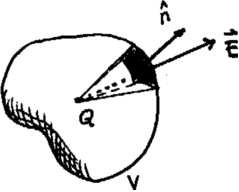
\includegraphics[width=0.35\textwidth]{images/fig_ft1_gauss.pdf}	 
% 	\end{center}
% 	\caption{}
% \end{figure} 




% \bibliographystyle{CBFT-apa-good}	% (uses file "apa-good.bst")
% \bibliography{CBFT.Referencias} % La base de datos bibliográfica

\end{document}
